% Options for packages loaded elsewhere
\PassOptionsToPackage{unicode}{hyperref}
\PassOptionsToPackage{hyphens}{url}
\PassOptionsToPackage{dvipsnames,svgnames*,x11names*}{xcolor}
%
\documentclass[
  10pt,
]{article}
\usepackage{lmodern}
\usepackage{setspace}
\usepackage{amssymb,amsmath}
\usepackage{ifxetex,ifluatex}
\ifnum 0\ifxetex 1\fi\ifluatex 1\fi=0 % if pdftex
  \usepackage[T1]{fontenc}
  \usepackage[utf8]{inputenc}
  \usepackage{textcomp} % provide euro and other symbols
\else % if luatex or xetex
  \usepackage{unicode-math}
  \defaultfontfeatures{Scale=MatchLowercase}
  \defaultfontfeatures[\rmfamily]{Ligatures=TeX,Scale=1}
  \setmainfont[]{DejaVu Serif}
  \setmonofont[]{DejaVu Sans Mono}
\fi
% Use upquote if available, for straight quotes in verbatim environments
\IfFileExists{upquote.sty}{\usepackage{upquote}}{}
\IfFileExists{microtype.sty}{% use microtype if available
  \usepackage[]{microtype}
  \UseMicrotypeSet[protrusion]{basicmath} % disable protrusion for tt fonts
}{}
\makeatletter
\@ifundefined{KOMAClassName}{% if non-KOMA class
  \IfFileExists{parskip.sty}{%
    \usepackage{parskip}
  }{% else
    \setlength{\parindent}{0pt}
    \setlength{\parskip}{6pt plus 2pt minus 1pt}}
}{% if KOMA class
  \KOMAoptions{parskip=half}}
\makeatother
\usepackage{xcolor}
\IfFileExists{xurl.sty}{\usepackage{xurl}}{} % add URL line breaks if available
\IfFileExists{bookmark.sty}{\usepackage{bookmark}}{\usepackage{hyperref}}
\hypersetup{
  colorlinks=true,
  linkcolor=red,
  filecolor=red,
  citecolor=red,
  urlcolor=red,
  pdfcreator={LaTeX via pandoc}}
\urlstyle{same} % disable monospaced font for URLs
\usepackage[margin=1cm,top=1cm,bottom=1cm,left=1cm,right=1cm,includeheadfoot]{geometry}
\usepackage{listings}
\newcommand{\passthrough}[1]{#1}
\lstset{defaultdialect=[5.3]Lua}
\lstset{defaultdialect=[x86masm]Assembler}
\usepackage{graphicx}
\makeatletter
\def\maxwidth{\ifdim\Gin@nat@width>\linewidth\linewidth\else\Gin@nat@width\fi}
\def\maxheight{\ifdim\Gin@nat@height>\textheight\textheight\else\Gin@nat@height\fi}
\makeatother
% Scale images if necessary, so that they will not overflow the page
% margins by default, and it is still possible to overwrite the defaults
% using explicit options in \includegraphics[width, height, ...]{}
\setkeys{Gin}{width=\maxwidth,height=\maxheight,keepaspectratio}
% Set default figure placement to htbp
\makeatletter
\def\fps@figure{htbp}
\makeatother
\setlength{\emergencystretch}{3em} % prevent overfull lines
\providecommand{\tightlist}{%
  \setlength{\itemsep}{0pt}\setlength{\parskip}{0pt}}
\setcounter{secnumdepth}{3}
% Enable graphics inclusion and ensure figure numbering works
\usepackage{graphicx}
\renewcommand{\figurename}{Figure}

% Configure fonts for Unicode support with fallbacks
\usepackage{newunicodechar}
\newunicodechar{⁴}{\textsuperscript{4}}
\newunicodechar{₄}{\textsubscript{4}}

% Enhanced code block styling for better contrast and readability
\usepackage{fancyvrb}
\usepackage{xcolor}
\usepackage{listings}

% Define custom colors for code blocks
\definecolor{codebg}{RGB}{245, 245, 245}      % Light gray background
\definecolor{codeborder}{RGB}{200, 200, 200}  % Medium gray border
\definecolor{codefg}{RGB}{50, 50, 50}         % Dark gray text

% Configure Verbatim environment for inline code
\DefineVerbatimEnvironment{Verbatim}{Verbatim}{%
    fontsize=\small,
    frame=single,
    framerule=0.5pt,
    framesep=3pt,
    rulecolor=\color{codeborder},
    bgcolor=\color{codebg},
    fgcolor=\color{codefg}
}

% Configure code block styling
\DefineVerbatimEnvironment{Highlighting}{Verbatim}{%
    fontsize=\footnotesize,
    frame=single,
    framerule=0.5pt,
    framesep=5pt,
    rulecolor=\color{codeborder},
    bgcolor=\color{codebg},
    fgcolor=\color{codefg}
}

% Style inline code with \texttt
\renewcommand{\texttt}[1]{%
    \colorbox{codebg}{\color{codefg}\ttfamily #1}%
}

% Configure listings package for code blocks
\lstset{
    backgroundcolor=\color{codebg},
    basicstyle=\footnotesize\ttfamily\color{codefg},
    breakatwhitespace=false,
    breaklines=true,
    captionpos=b,
    commentstyle=\color{codefg},
    deletekeywords={...},
    escapeinside={\%*}{*)},
    extendedchars=true,
    frame=single,
    framerule=0.5pt,
    framesep=5pt,
    keepspaces=true,
    keywordstyle=\color{codefg},
    language=Python,
    morekeywords={*,...},
    numbers=left,
    numbersep=5pt,
    numberstyle=\tiny\color{codefg},
    rulecolor=\color{codeborder},
    showspaces=false,
    showstringspaces=false,
    showtabs=false,
    stepnumber=1,
    stringstyle=\color{codefg},
    tabsize=2,
    title=\lstname
}

% Override any Pandoc default lstset configurations
\AtBeginDocument{
    \lstset{
        backgroundcolor=\color{codebg},
        basicstyle=\footnotesize\ttfamily\color{codefg},
        frame=single,
        framerule=0.5pt,
        framesep=5pt,
        rulecolor=\color{codeborder},
        numbers=left,
        numbersep=5pt,
        numberstyle=\tiny\color{codefg}
    }
}

% Configure hyperref colors consistently
\AtBeginDocument{
% Override pandoc's hidelinks setting with consistent options
\hypersetup{
    colorlinks=true,
    allcolors=red,
    linkcolor=red,
    urlcolor=red,
    citecolor=red,
    filecolor=red,
    menucolor=red,
    linktoc=all
}
}

\title{Appendix: Free Energy and Active Inference}
\author{Daniel Ari Friedman\\ ORCID: 0000-0001-6232-9096\\ Email: daniel@activeinference.institute}
\date{August 15, 2025}

\begin{document}
\maketitle

{
\hypersetup{linkcolor=black}
\setcounter{tocdepth}{3}
\tableofcontents
}
\setstretch{1.0}
\hypertarget{appendix-the-free-energy-principle-and-active-inference}{%
\section{Appendix: The Free Energy Principle and Active
Inference}\label{appendix-the-free-energy-principle-and-active-inference}}

\hypertarget{overview}{%
\subsection{Overview}\label{overview}}

The Free Energy Principle (FEP) posits that biological systems maintain
their states by minimizing variational free energy, thereby reducing
surprise via prediction and model updating. Active Inference extends
this by casting action selection as inference under prior preferences.
Background: see the concise overview on the
\href{https://en.wikipedia.org/wiki/Free_energy_principle}{Free energy
principle} and the monograph
\href{https://direct.mit.edu/books/oa-monograph/5299/Active-InferenceThe-Free-Energy-Principle-in-Mind}{Active
Inference (MIT Press)}.

This appendix emphasizes relationships among: (i) the four-fold
partition of Active Inference, (ii) Quadrays (Fuller.4D) as a geometric
scaffold for mapping this partition, and (iii) information-geometric
flows (Einstein.4D analogy) that underpin perception--action updates.
For the naming of 4D namespaces used throughout---Coxeter.4D (Euclidean
E4), Einstein.4D (Minkowski spacetime analogy), Fuller.4D
(Synergetics/Quadrays)---see
\passthrough{\lstinline!02\_4d\_namespaces.md!}.

\hypertarget{mathematical-formulation-and-equation-callouts-equations-linkage}{%
\subsection{Mathematical Formulation and Equation Callouts (Equations
linkage)}\label{mathematical-formulation-and-equation-callouts-equations-linkage}}

\begin{itemize}
\item
  Variational free energy (discrete states) --- see Eq.
  \eqref{eq:supp_free_energy} in the equations appendix, implemented by
  \href{08_equations_appendix.md\#code:free_energy}{\passthrough{\lstinline!free\_energy!}}:

  \begin{equation}\label{eq:free_energy_appendix_ref}
  \mathcal{F} = -\log P(o\mid s) + \mathrm{KL}\big[ Q(s)\;\|\; P(s) \big]
  \end{equation}

  where \(Q(s)\) is a variational posterior, \(P(s)\) a prior, and
  \(P(o\mid s)\) the likelihood. Lower \(\mathcal{F}\) is better.
\item
  Fisher Information Matrix (FIM) as metric --- see Eq.
  \eqref{eq:supp_fim} in the equations appendix and
  \href{08_equations_appendix.md\#code:fisher_information_matrix}{\passthrough{\lstinline!fisher\_information\_matrix!}}:

  \begin{equation}\label{eq:fim_definition}
  F_{i,j} = \mathbb{E}\left[ \partial_{\theta_i} \log p(x;\theta)\; \partial_{\theta_j} \log p(x;\theta) \right].
  \end{equation}
\item
  Natural gradient descent under information geometry --- see Eq.
  \eqref{eq:supp_natgrad} in the equations appendix and
  \href{08_equations_appendix.md\#code:natural_gradient_step}{\passthrough{\lstinline!natural\_gradient\_step!}};
  overview:
  \href{https://en.wikipedia.org/wiki/Natural_gradient}{Natural
  gradient}:

  \begin{equation}\label{eq:natural_gradient_update}
  \theta \leftarrow \theta - \eta\, F(\theta)^{-1}\, \nabla_{\theta} L(\theta).
  \end{equation}
\end{itemize}

Figures: See the Fisher Information Matrix and free energy figures in
the optimization section above.

Discrete variational optimization on the quadray lattice:
\passthrough{\lstinline!discrete\_ivm\_descent!} greedily descends a
free-energy-like objective over IVM moves, yielding integer-valued
trajectories. See the path animation artifact
\passthrough{\lstinline!discrete\_path.mp4!} in
\passthrough{\lstinline!quadmath/output/!}.

\begin{figure}
\centering
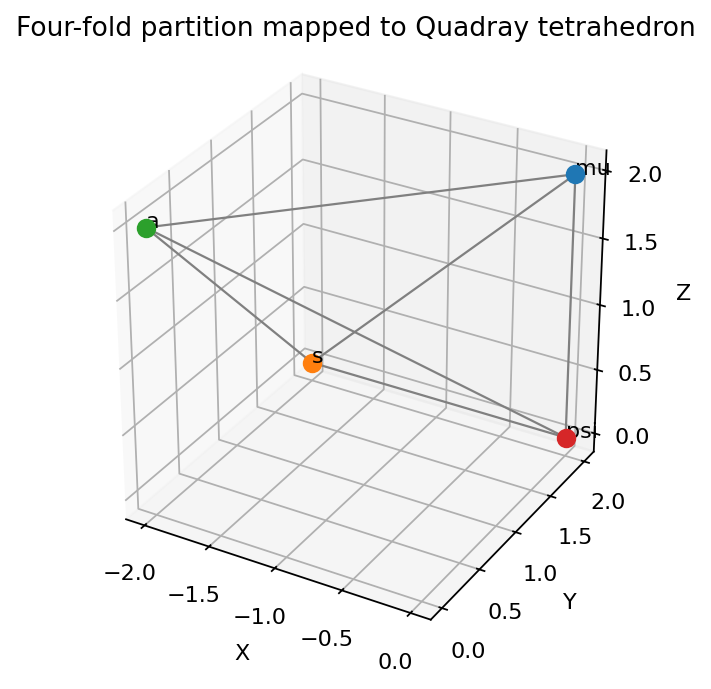
\includegraphics{../output/figures/partition_tetrahedron.png}
\caption{\textbf{Active Inference four-fold partition mapped to a
Quadray tetrahedron in Fuller.4D}. This 3D tetrahedral visualization
demonstrates the geometric embedding of Active Inference's fundamental
four-fold partition within the Quadray coordinate system.
\textbf{Tetrahedral structure}: The four vertices of the regular
tetrahedron represent the four components of the Active Inference
framework: perception, action, internal states, and external states.
\textbf{Partition mapping}: Each face of the tetrahedron corresponds to
a specific partition of the four-fold system, with the edges
representing the relationships and interactions between different
components. \textbf{Fuller.4D significance}: This geometric
representation leverages the tetrahedral nature of Quadray coordinates
to provide an intuitive visualization of the Active Inference
framework's structure. The tetrahedron serves as a natural container for
the four-fold partition, emphasizing the interconnected nature of
perception, action, and state representation in active inference.
\textbf{Optimization context}: The tetrahedral geometry also suggests
natural optimization strategies that respect the four-fold structure,
potentially leading to more efficient inference algorithms that leverage
the geometric relationships between different components. This
visualization demonstrates how the Fuller.4D framework can provide
insights into complex systems like Active Inference through geometric
intuition.}
\end{figure}

\hypertarget{four-fold-partition-and-tetrahedral-mapping-quadrays-fuller.4d}{%
\subsection{Four-Fold Partition and Tetrahedral Mapping (Quadrays;
Fuller.4D)}\label{four-fold-partition-and-tetrahedral-mapping-quadrays-fuller.4d}}

Active Inference partitions the agent--environment system into four
coupled states:

\begin{itemize}
\tightlist
\item
  Internal (\(\mu\)) --- agent's internal states
\item
  Sensory (\(s\)) --- observations
\item
  Active (\(a\)) --- actions
\item
  External (\(\psi\)) --- latent environmental causes
\end{itemize}

See, for an overview of this partition and generative process
formulations, the
\href{https://discovery.ucl.ac.uk/id/eprint/10176959/1/1-s2.0-S1571064523001094-main.pdf}{Active
Inference review} and the general entry on
\href{https://en.wikipedia.org/wiki/Active_inference}{Active inference}.

Tetrahedral mapping via Quadrays (Fuller.4D): assign each state to a
vertex of a tetrahedron, using Quadray coordinates
\passthrough{\lstinline!(A,B,C,D)!} with non-negative components and at
least one zero after normalization. One canonical mapping is
\passthrough{\lstinline!A \\leftrightarrow Internal (\\mu)!},
\passthrough{\lstinline!B \\leftrightarrow Sensory (s)!},
\passthrough{\lstinline!C \\leftrightarrow Active (a)!},
\passthrough{\lstinline!D \\leftrightarrow External (\\psi)!}. The edges
capture the pairwise couplings (e.g.,
\passthrough{\lstinline!\\mu\\text\{--\}s!} for perceptual inference;
\passthrough{\lstinline!a\\text\{--\}\\psi!} for control). Integer
tetravolume then quantifies the ``coupled capacity'' region spanned by
jointly feasible states in a time slice; see
\passthrough{\lstinline!Quadray!} and tetravolume methods in
\passthrough{\lstinline!03\_quadray\_methods.md!}.

Interpretation note: this Quadray-based mapping is a didactic geometric
scaffold. It is not standard in the Active Inference literature, which
typically develops the four-state partition in probabilistic graphical
terms. Our use highlights structural symmetries and discrete volumetric
quantities available in Fuller.4D, building on the computational
foundations developed in the
\href{https://github.com/4dsolutions}{4dsolutions ecosystem} for
tetrahedral modeling and volume calculations. See the
\href{07_resources.md}{Resources} section for comprehensive details on
the computational implementations.

Code linkage (no snippet): see
\passthrough{\lstinline!example\_partition\_tetra\_volume!} in
\passthrough{\lstinline!src/examples.py!} and the partition tetrahedron
figure above.

\hypertarget{how-the-4d-namespaces-relate-here}{%
\subsection{How the 4D namespaces relate
here}\label{how-the-4d-namespaces-relate-here}}

\begin{itemize}
\tightlist
\item
  Fuller.4D (Quadrays): geometric embedding of the four-state partition
  on a tetrahedron; integer tetravolumes and IVM moves provide discrete
  combinatorial structure.
\item
  Coxeter.4D (Euclidean E4): exact Euclidean measurements (e.g.,
  Cayley--Menger determinants) for tetrahedra underlying volumetric
  comparisons and scale relations.
\item
  Einstein.4D (Minkowski analogy): information-geometric flows (natural
  gradient, metric-aware updates) supply a continuum picture for
  perception--action dynamics.
\end{itemize}

The three roles are complementary: Fuller.4D encodes partition
structure, Coxeter.4D provides exact metric geometry for static
comparisons, and Einstein.4D guides dynamical descent.

\hypertarget{joint-optimization-in-the-tetrahedral-framework-methods-linkage}{%
\subsection{Joint Optimization in the Tetrahedral Framework (Methods
linkage)}\label{joint-optimization-in-the-tetrahedral-framework-methods-linkage}}

\begin{itemize}
\tightlist
\item
  Perception: update \(\mu\) to minimize prediction error on \(s\) under
  the generative model (descending \(\nabla_{\mu} F\)).
\item
  Action: select \(a\) that steers \(\psi\) toward preferred outcomes
  (descending \(\nabla_{a} F\)).
\end{itemize}

Continuous-time flows (Einstein.4D analogy for metric/geodesic
intuition): see \passthrough{\lstinline!perception\_update!} and
\passthrough{\lstinline!action\_update!} in
\passthrough{\lstinline!src/information.py!}. Discrete Quadray moves
connect to these flows via greedy descent on a local free-energy-like
objective; see \passthrough{\lstinline!discrete\_ivm\_descent!} in
\passthrough{\lstinline!src/discrete\_variational.py!} and the path
artifacts in \passthrough{\lstinline!quadmath/output/!}.

\hypertarget{neuroscience-and-predictive-coding}{%
\subsection{Neuroscience and Predictive
Coding}\label{neuroscience-and-predictive-coding}}

Under Active Inference, cortical circuits minimize free energy through
recurrent exchanges of descending predictions and ascending prediction
errors, aligning with predictive coding accounts. See the neural
dynamics framing in \href{https://arxiv.org/abs/2001.08028}{Active
Inference neural dynamics (arXiv:2001.08028)}.

\hypertarget{relation-to-reinforcement-learning-and-control}{%
\subsection{Relation to Reinforcement Learning and
Control}\label{relation-to-reinforcement-learning-and-control}}

Active Inference replaces explicit value functions with prior
preferences over outcomes and transitions, balancing exploration
(epistemic value) and exploitation (pragmatic value) via expected free
energy. See \href{https://arxiv.org/abs/2002.12636}{Active Inference and
RL (arXiv:2002.12636)}. Connections to optimal control arise when
minimizing expected free energy plays the role of a control objective;
cf.~\href{https://en.wikipedia.org/wiki/Optimal_control}{Optimal
control}.

\hypertarget{links-to-other-theories}{%
\subsection{Links to Other Theories}\label{links-to-other-theories}}

\begin{itemize}
\tightlist
\item
  Bayesian Brain hypothesis:
  \href{https://en.wikipedia.org/wiki/Bayesian_brain}{Bayesian brain}
\item
  Predictive Coding:
  \href{https://en.wikipedia.org/wiki/Predictive_coding}{Predictive
  coding}
\item
  Information Geometry:
  \href{https://en.wikipedia.org/wiki/Fisher_information}{Fisher
  information},
  \href{https://en.wikipedia.org/wiki/Natural_gradient}{Natural
  gradient}
\end{itemize}

\hypertarget{implications-for-ai-and-robust-computation}{%
\subsection{Implications for AI and Robust
Computation}\label{implications-for-ai-and-robust-computation}}

FEP/Active Inference provide algorithms that unify perception and action
under uncertainty, offering biologically plausible alternatives to
standard RL with adaptive exploration and robust decision-making. See
\href{https://arxiv.org/abs/1907.03876}{applications in AI
(arXiv:1907.03876)}.

\hypertarget{code-reproducibility-and-cross-references}{%
\subsection{Code, Reproducibility, and
Cross-References}\label{code-reproducibility-and-cross-references}}

-- Equation references:
\href{08_equations_appendix.md\#eq:free_energy}{Eq. (Free Energy)},
\href{08_equations_appendix.md\#eq:fim}{Eq. (FIM)},
\href{08_equations_appendix.md\#eq:natgrad}{Eq. (Natural Gradient)} in
\passthrough{\lstinline!08\_equations\_appendix.md!}. -- Code anchors
(for readers who want to run experiments):
\href{03_quadray_methods.md\#code:free_energy}{\passthrough{\lstinline!free\_energy!}},
\href{03_quadray_methods.md\#code:fisher_information_matrix}{\passthrough{\lstinline!fisher\_information\_matrix!}},
\href{03_quadray_methods.md\#code:natural_gradient_step}{\passthrough{\lstinline!natural\_gradient\_step!}},
\passthrough{\lstinline!perception\_update!},
\passthrough{\lstinline!action\_update!}, and
\passthrough{\lstinline!discrete\_ivm\_descent!} in
\passthrough{\lstinline!src/information.py!} and
\passthrough{\lstinline!src/discrete\_variational.py!}.

Demo and figures generated by
\passthrough{\lstinline!quadmath/scripts/information\_demo.py!} output
to \passthrough{\lstinline!quadmath/output/!}:

\begin{itemize}
\tightlist
\item
  \textbf{Visualizations}:
  \passthrough{\lstinline!fisher\_information\_matrix.png!},
  \passthrough{\lstinline!fisher\_information\_eigenspectrum.png!},
  \passthrough{\lstinline!natural\_gradient\_path.png!},
  \passthrough{\lstinline!free\_energy\_curve.png!},
  \passthrough{\lstinline!partition\_tetrahedron.png!}.
\item
  \textbf{Raw data}:
  \passthrough{\lstinline!fisher\_information\_matrix.csv!},
  \passthrough{\lstinline!fisher\_information\_matrix.npz!} (F, grads,
  X, y, w\_true, w\_est),
  \passthrough{\lstinline!fisher\_information\_eigenvalues.csv!},
  \passthrough{\lstinline!fisher\_information\_eigensystem.npz!}.
\item
  \textbf{External validation}: Cross-reference with volume calculations
  and tetrahedral modeling tools from the
  \href{https://github.com/4dsolutions}{4dsolutions ecosystem}. See the
  \href{07_resources.md}{Resources} section for comprehensive details.
\end{itemize}

\end{document}
